\section{Das Projekt: iFMS@Salesforce}
%\section{Forschungsergebnisse}
\label{cha:result}
\begin{comment}
In Kapitel „Forschungsergebnisse“ stellen Sie die Ergebnisse ihrer Arbeit dar.
An dieser Stelle nehmen Sie noch keine Interpretation oder Erläuterung der 
Ergebnisse vor, sondern beschreiben rein deskriptiv ihre Befunde. Eine 
Auswertung findet im nachfolgenden Kapitel statt.
\end{comment}
Mit dem entwickelten 
Vorgehensmodell soll nun 
beispielthaft die Cloud-Migration 
des in Kapitel~\ref{cha:replyundifms} vorgestellten iFMS theoretisch geplant 
werden. In Kapitel~\ref{cha:diskussion} wird der entstandene Plan mit dem 
Vorgehen aus der Praxis verglichen und diskutiert.

Die Cloudversion dieser Software wird hier "`iFMS@Salesforce"' genannt und von 
iFMS abgegrenzt. Aus dem Namen geht die gewählte Cloud-Plattform hervor -- eine 
strategische Entscheidung, die ebenfalls im Kapitel~\ref{cha:replyundifms} begründet wurde.

\subsection{Phase I: Entwickeln einer Vision}
Um zu der Produktvision zu gelangen, dienen die in 
Kapitel~\ref{cha:entwicklung_vorgehensmodell} identifizierten Chancen und 
Risiken als Checkliste bei einem Brainstorming. Das Ergebnis sind Epics, 
grobgranulare, funktionale und nicht-funktionale Anforderungen an die neue 
Software \pcite{}{}{10_tips_for_writing_good_user_stories}.
Im Wechselspiel mit den gesammelten Epics werden Geschäftsmodell und Strategie 
definiert. Einige Chancen und Risiken ziehen strategische Implikationen mit 
sich, andere Chancen werden durch eine gewählte Strategie ausgeschlossen. Zum 
Beispiel können gewisse Chancen die Erschließung neuer Märkte ermöglichen oder aber 
eine Realisierung derselben aus strategischen Gründen ausschließen. 

In dieser Arbeit liegt der Schwerpunkt auf dem Modell, das den Weg zur Vision 
beschreibt -- nicht auf der iFMS@Salesforce-Vision selbst, die aus Sicht des 
Autors  keinen allgemeinen Mehrwert besitzt. Deshalb wird dieser Weg 
hier dargestellt, auf eine vollständige Beschreibung der Vision jedoch 
verzichtet. 
\subsubsection{Realisierung von Chancen}
\begin{description}
	\item[Soziales Element: Vernetzung und Einbeziehung von Nutzern] Die 
Vernetzung zwischen den Nutzern einer Firma erfolgt über Chatter, dem 
Salesforce Äquivalent von Facebook. Der ISV bietet Kundensupport über die 
Salesforce Service Cloud. Entwickler sind für Kunden direkter erreichbar. Durch 
die dort gesammelten Erfahrung können zukünftige Entwicklungsarbeiten 
zielgerichteter erfolgen. Kunden sollen das Gefühl bekommen, 
dass ihr Anliegen durch den Support schnell und zufriedenstellend gelöst 
wird. Durch die schnelle Umsetzung von eingebrachten 
Verbesserungsvorschlägen, soll sich der Eindruck festigen, dass jeder 
Kunde aktiv am Produkt mitentwickeln kann und sich selbst im Produkt wieder 
findet.
	\item[Analysemöglichkeiten] Der ISV hat Zugriff auf die 
Salesforceinstanzen seiner Kunden. Dadurch kann er Fehlkonfigurationen 
und Fehlbedienungen erkennen, Supportangebote verbessern oder 
Benutzeroberflächen intuitiver gestalten. Der ISV kann ebenfalls analysieren, 
welche Funktionen besonders häufig genutzt werden und die zugehörigen Abläufe 
verbessern oder automatisieren.
	\item[Mobile Nutzung] Mit der Mobile App Salesforce1 ist die Salesforce 
Anwendung auch auf Mobilgeräten nutzbar. Damit ein echter Mehrwert für 
den Kunden entsteht, sollen sich
\begin{itemize}
	\item Rauminformationen wie Belegungen und Ansprechpartner abrufen 
lassen.
	\item Räume buchen lassen.
	\item Schadensmeldungen eingeben lassen. Die Freigabe durch den 
verantwortlichen Mitarbeiter resultiert in einem Auftrag an einen Dienstleister 
zur Schadensbehebung.
	\item über Anwesenheitserkennung Raumtemperatur und Licht regeln lassen.
	\item Räume über ein Indoornavigationssystem finden lassen.
	\item Reiningungspläne einsehen und ändern, sowie Sonderreinigungen 
anfordern lassen.
	\item erfolgte Dienstleistungen wie Reinigungen, Reparaturen oder 
Caterings bewerten lassen, um die Auswahl künftiger Dienstleister besser zu 
gestalten.
\end{itemize}

	\item[Reduzierte Markteintrittskosten \& Skalierte Märkte] Um die 
Hürden für potentielle Kunden gering zu halten und das Produkt auf diese Weise 
auch für kleine und mittlere Unternehmen attraktiv zu machen, ist die 
SAP- und CAD-Anbindung optional. Durch die Nutzung des Salesforce Marktplatzes 
für Apps können Kunden das Produkt leicht beziehen und in einer Basisversion 
testen beziehungsweise nutzen. \\
Die Erschließung globaler Märkte erfolgt einerseits über den Marktplatz, 
andererseits über die gezielte Ansprache großer, internationaler Unternehmen, 
um iFMS@Salesforce langfristig international zu etablieren.

	\item[Skalierung der Leistung] Raumbelegungen lassen sich über die 
verfügbare Leistung in akzeptabler Zeit in verschiedenen 
Dimensionen optimieren. \\
CAD-Pläne werden nicht mehr lokal sondern in der Cloud 
konvertiert.

	\item[Time to market \& kürzere Releasezyklen] Eine vermarktbare 
Basisversion mit einem Bruchteil der Funktionalitäten der komplexen 
Altsoftware soll rasch entwickelt, vermarktet und genutzt werden, um bei 
Verhandlungen mit Neu- und Altkunden Interesse zu wecken. \\
Durch die langjährige Erfahrung mit CAD und SAP sollen in Zusammenarbeit mit in 
Salesforce erfahrenen Kollegen, die Kernkompetenzen zügig in die Cloud 
übertragen werden.
	\item[Alternativen am Kunden testen] Die Kultur 
des Mitentwickelns (siehe Abschnitt zur Einbeziehung von Nutzern oben) soll 
genutzt werden, um es interessierten Powerusern in Sandboxes zu ermöglichen den aktuellen 
Entwicklungsstand zu testen und direktes Feedback zu geben, das in die nächsten 
Sprintplanungen einfließen kann.
	\item[Wartung einer einzigen Version] Der Wartungsaufwand soll 
reduziert werden, indem es jeweils nur eine Version der Basis-, SAP- und 
CAD-Komponenten gibt. Anpassungen werden dem Kunden als Zusatzdienstleistung 
verkauft, sodass zusätzlicher Wartungsaufwand zu zusätzlichen Umsätzen für den 
 ISV führt.
	\item[Standardisierte Komponenten] Standardisierte Komponenten lassen 
sich auf dem Salesforce App Marktplatz beziehen. Beispiel dafür ist die 
nahtlose Anbindung an Amazons Dateispeicher S3, um es Kunden zu ermöglichen 
Dateien zu Liegenschaften oder Verträgen zu hinterlegen. Da der ISV keine 
Kernkompetenz beim Bearbeiten von CAD-Plänen besitzt, soll eine entsprechende 
Komponente aus dem Marktplatz bezogen werden, sodass der Kunde für keinen 
Prozess iFMS@Salesforce verlassen muss.
	\item[Stetige Umsätze] Durch ein Preismodell in dem pro Nutzer und 
Monat bei einer Mindestlaufzeit von einem Jahr abgerechnet wird, lassen sich 
stetige Umsätze generieren, die dem ISV mehr Planungssicherheit geben.
	\item[Verkauf an Fachabteilungen] Im Marketing soll ein Schwerpunkt 
darauf gelegt werden, Fachabteilungen direkt zu erreichen, zum Beispiel bei 
Fachtagungen einschlägiger Themen. Idealerweise lassen sich kleine Firmen 
erreichen, die das Thema Liegenschaftsmanagement bisher ohne 
Softwareunterstützung bewältigt haben. Sind Fachabteilungen überzeugt lässt 
sich das Produkt ohne Eingriffe in die IT-Landschaft vor Ort nutzen; eine 
Einbeziehung der IT-Abteilung ist nicht mehr oder nur in geringem Umfang nötig.
\end{description}
\subsubsection{Vermeidung von Risiken}
\begin{description}
	\item[Hohe Kosten durch Pay-per-Use] Salesforce rechnet pro Nutzer und 
Monat ab, sodass weder für den ISV noch für den Kunden mit 
unerwartet hohen Kosten zu rechnen ist.
	\item[Lock-in Effekte] Arlanis Reply hat sich strategisch an Salesforce 
gebunden; der Lock-in Effekt wird in Kauf genommen.
	\item[Komplexität unbedacht gekoppelter Komponenten] Bei Bezug 
von Komponenten aus dem Salesforce Marktplatz wird darauf geachtet nur aktiv 
gepflegte Komponenten mit einem hohen Reifegrad auszuwählen. Außerdem soll vor 
der Wahl einer bestimmten Komponente die Komplexität des Gesamtsystems in einer 
Kosten-Nutzen-Analyse betrachtet werden.
	\item[Datenmigration] Zahlen- und Mengenmäßige Zugriffsbeschränkungen 
auf die Datenbank durch Salesforce könnten eine schrittweise Migration der 
Daten erforderlich machen. Um den Parallelbetrieb mit dem Altsystem so kurz wie 
möglich zu halten, soll ein leicht zu verstehendes Konzept erarbeitet und 
implementiert werden, mit dem ein zügiger Umzug von logischen Teilkomponenten, 
wie Etagen, Standorten oder Ländern ermöglicht wird.
	\item[Leistungstransparenz] Um potentielle Kunden, die iFMS@Salesforce 
in der Basisversion testen, vom Produkt zu überzeugen, sollen bei der 
Entwicklung Schwerpunkte auf eine intuitive Bedienung und begeisternde Features 
gelegt werden.
	\item[Geringere Umsätze] Auch das bisherige Geschäftsmodell sah 
einmalige Zahlungen für die Installation und Anpassung sowie fortlaufende Zahlungen 
für die Nutzung vor. Daher besteht dieses Risiko nicht. 
	\item[Geringere Anpassbarkeit] Mit Force.com und Heroku wird Salesforce 
zu einem PaaS-Dienstleister. Features, die sich mit der 
Kernfunktionalität oder Erweiterungen von Salesforce nicht umsetzen lassen, 
lassen sich auf diese Weise nahezu ohne Einschränkungen realisieren.
	\item[Organisatorische und strukturelle Umbrüche] Die Einarbeitungszeit 
des alten iFMS-Teams in die Cloud-Technologie soll durch eine 
Team-Zusammensetzung mit erfahrenen Salesforce-Entwicklern und -Beratern 
reduziert werden. \\
Da sowohl Arlanis Reply und Syskoplan Reply als Tochtergesellschaften bereits 
eng vernetzt sind, ergeben sich wenige strukturelle Änderungen. Es muss 
allerdings darauf geachtet werden, dass das alte iFMS-Team trotz totaler Abkehr 
von der bisher genutzten Technologie im neuen Team und im neuen Produkt 
aufgeht.
	\item[Updatefrequenz erfordert Agilität] Bisherige Ansätze der agilen 
Entwicklung werden systematisch mit neuen Entwicklungen im Bereich des Software 
Engineerings und des Projektmanagements verglichen und gegebenenfalls 
angepasst. Die Einbeziehung der Nutzer in die Entwicklung macht eine 
Berücksichtigung ihrer Anliegen in der Sprintplanung in besonderem Maße 
erforderlich.
\end{description}

\subsubsection{Geschäftsmodell \& Strategie}
Die stratetischen Implikationen einzelner Chancen und Risiken treten deutlich 
hervor; sie beeinflussen die klassischen "`Vier Ps"' des Marketingmixes und 
spiegeln sie wider \pcite{}{1003}{marketingmanagement}:
\begin{description}
	\item[Product -- Produktpolitik] Wie soll das 
zukünftige Produkt iFMS@Salesforce aussehen? Mit welcher Technik, in welcher 
Qualtität und in Verbindung mit welchen zusätzlichen Dienstleistungen soll es 
umgesetzt und angeboten werden?
	\item[Price -- Preispolitik] Welchen Preis sind die 
Kunden bereit für die Basis-Version, welchen für CAD- und SAP-Unterstützung zu zahlen? 
Welches Preismodell wird gewählt (siehe Kapitel~\ref{cha:isv})? 
	\item[Promotion -- Kommunikationspolitik] Wie werden (Neu-)Kunden 
erreicht und dauerhaft gewonnen? Wie wird die Kommunikationspolitik durch das 
soziale Element der Cloud unterstützt?
	\item[Place --  Distributionspolitik] Gelangt iFMS@Salesforce über den 
Salesforce Marktplatz zum Kunden oder wird das Produkt für den Kunden in seiner 
Salesforce-Instanz aufgesetzt und angepasst?
\end{description}
Die Festlegung von Strategie, Marketing und Geschäftsmodell muss daher unter 
besonderer Beachtung der genannten Aspekte erfolgen. 

\begin{comment}
In Orientierung an Abbildung~\ref{fig:einfluss_des_preises_auf_business} soll 
in Tabelle~\ref{} zunächst iFMS in Preis und davon abhängigen Dimensionen 
analysiert werden. 


\begin{table}[bh]
\newcommand{\colBreite}{0.135\textwidth}
\newcommand{\theColor}{blue!25}
\centering
\begin{tabular}[width=0.95\textwidth]
{|p{\colBreite}|p{\colBreite}|p{\colBreite}|p{\colBreite}|p{
\colBreite} |p{\colBreite}|}
\hline
\textbf{Verkaufs\-preis} & \textbf{Kosten für Kun\-den\-aqui\-si\-tion} & 
\textbf{Vertrieb} & \textbf{Kun\-den\-be\-ziehungen} & \textbf{Vertretbare 
Nutzerschulungen} & \textbf{Ziel\-gruppen} \\
\hline
€€€€€ & Hoch & Extern & \cellcolor{\theColor}Persönlich\newline iFMS & 
\cellcolor{\theColor}Erheblich\newline iFMS & 
\cellcolor{\theColor}Unterneh\-men\newline iFMS \\
\hline
\cellcolor{\theColor}€€€\newline iFMS & \cellcolor{\theColor}Moderat\newline 
iFMS & \cellcolor{\theColor}Intern\newline iFMS & Telefonisch & Moderat & 
Abteilungen, 
KMU \\
\hline
€ & Niedrig & Keinen & Web & Minimal & KMU, Personen \\
\hline
\end{tabular}
\caption{Kosten für iFMS und iFMS@Salesforce aus Kundensicht und Folgerungen 
auf die Zielgruppe.}
\label{tab:analyse_preis}
\end{table}

Die Bedeutung für das Geschäftsmodell und die Strategie soll beispielhaft an 
einem Aspekt gezeigt werden, der Zielgruppe. Die Zielgruppe von iFMS bestand 
aus großen Unternehmen mit einer bestimmten 
Zahl von Liegenschaften, für deren Verwaltung sich Einrichtungs-, Wartungs- und 
Schulungsaufwände lohnen. Die Beschränkung auf diese Zielgruppe ließe sich 
falls gewünscht mit den Mitteln der Cloud aufheben. Eine Basisversion könnte 
durch eine einfache Installation und begeisternde Cloud-Features zu einer 
relativ niedrigen monatlichen Gebühr in einer Art Freemium-Modell Neukunden 
erreichen. Die Unterstützung für SAP und CAD, spezielle Anpassungen der 
Software, Integration weiterer Systeme, Support sowie Schulungen ließen sich 
durch Kunden hinzubuchen und machten die Hauptumsatzquelle für das Unternehmen 
aus. Dabei wäre darauf zu achten, den persönlichen Kontakt zu Kunden nicht zu 
verlieren: Das Verarbeiten von CAD-Plänen mit sicherheitsrelevanten Daten oder 
Finanzdaten aus SAP mit personenbezogenen Daten in der Cloud und macht es 
erforderlich, dass der Kunde Salesforce und dem ISV vertraut.
\end{comment}
\subsection{Phase II: Machbarkeitsstudie}
Die Machbarkeitsstudie untersucht die Vision, die ein strategisches Ziel und 
eine weitgehend ungeordnete Menge von Anforderungen beinhaltet. Dabei sollen 
die Epics, die im Sinne der Strategie ausgewählt wurden, auf ihre technische 
und wirtschaftliche Machbarkeit geprüft werden.
\usetikzlibrary{decorations.text}
\usetikzlibrary{calc}
\usetikzlibrary{fit}
\usetikzlibrary{shapes}
\usetikzlibrary{arrows,positioning} 

%\begin{document}
\begin{figure}[h]
\begin{center}
\scalebox{1}{
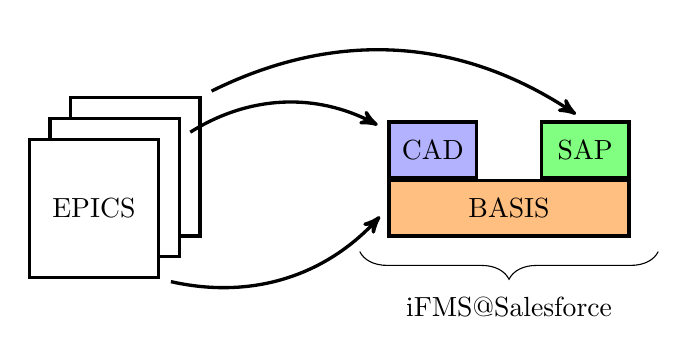
\begin{tikzpicture}[
    scale=5,
    pile/.style={thick, ->, >=stealth', shorten <=2pt, shorten
    >=2pt},
    punkt/.style={
           rectangle,
           draw=black, very thick,
           text width=8em,
           minimum height=2em,
           text centered},
    ]

\newcommand{\size}{1.5}
\coordinate (SW) at (0,0);
\coordinate (SE) at (\size,0);
\coordinate (NW) at (0,\size);
\coordinate (NE) at (\size,\size);

% axis
\newcommand{\cBasis}{orange!50}
\newcommand{\cCAD}{blue!30}
\newcommand{\cSAP}{green!50}

% iFMS@Salesforce
\node[punkt,fill=\cBasis] (BASIS) at (0,0) {BASIS};
\node[punkt,fill=\cCAD,text width=2.5em,anchor=south west] (CAD) at 
(BASIS.north west) {CAD};
\node[punkt,fill=\cSAP,text width=2.5em,anchor=south east] (SAP) at (BASIS.north 
east) {SAP};
;

% Klammer
\draw 
[decorate,decoration={brace,amplitude=10pt,mirror},xshift=-4pt,yshift=-200pt]
([yshift=-1pt,xshift=-2pt]BASIS.south west) -- 
([yshift=-1pt,xshift=2pt]BASIS.south east) node [black,midway,yshift=-20pt] 
{iFMS@Salesforce};

\coordinate (EPICS) at (-3em,0);
\newcommand{\epicsXShift}{0.15em}
\newcommand{\epicsYShift}{0.15em}
\node[punkt,text width=4em,minimum height=5em,fill=white] (E3) at ($ (EPICS) + 
(2*\epicsXShift,2*\epicsYShift) $) {};
\node[punkt,text width=4em,minimum height=5em,fill=white] (E2) at ($ (EPICS) + 
(\epicsXShift,\epicsYShift) $) {};
\node[punkt,text width=4em,minimum height=5em,fill=white] (EPICS) at (EPICS) 
{EPICS};

% Pfeile
\path[very thick, ->, >=stealth', shorten <=4pt, shorten >=4pt]
    (EPICS.south east) edge[bend right] node [right] {} (BASIS.west)
    (E2) edge[bend left] node [right] {} (CAD)
    (E3.north east) edge[bend left] node [left] {} (SAP.north);

\end{tikzpicture}
}
\caption{Schematische Darstellung der Zuordnung von Epics}
\label{fig:epics_to_components}
\end{center}
\end{figure}

Wie in Abbildung~\ref{fig:epics_to_components} dargestellt soll iFMS@Salesforce 
aus drei Versionen bestehen: der Basis-Version sowie der CAD- und der 
SAP-Erweiterung. Aus der strategischen Ausrichtung heraus werden nun den 
Versionen Epics zugeordnet, sowie Funktionen die unbedingt notwendig sind um die 
jeweilige Version zu vermarkten. Der Preis -- ob Verkaufspreis oder 
Lizenzierungskosten -- kann aufgrund der langjährigen Erfahrung im 
On-Premise-Geschäft gut abgeschätzt werden. Aus dieser Erfahrung oder den direkten 
Gesprächen heraus können die im Vertrieb tätigen Mitarbeiter, auch die 
Bereitschaft der Kunden abschätzen, den Weg in die Cloud mitzugehen. Die 
Salesforce- und iFMS-Entwickler bei Reply schätzen nun in einem ersten Schritt 
die grundsätzliche technische Umsetzbarkeit ein.

\usetikzlibrary{decorations.text}
\usetikzlibrary{calc}
\usetikzlibrary{fit}
\usetikzlibrary{shapes}
\usetikzlibrary{arrows,positioning} 

%\begin{document}
\begin{figure}[h]
\begin{center}
\scalebox{0.9}{
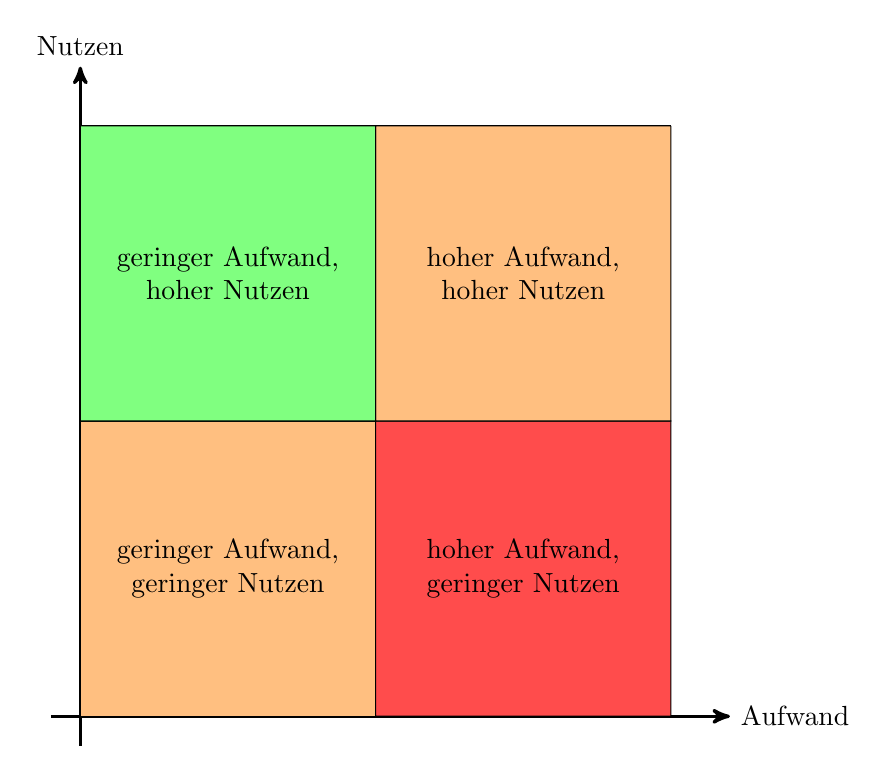
\begin{tikzpicture}[
    scale=5,
    axis/.style={very thick, ->, >=stealth'},
    important line/.style={thick},
    dashed line/.style={dashed, thin},
    pile/.style={thick, ->, >=stealth', shorten <=2pt, shorten
    >=2pt},
    text/.style={},
    every node/.style={color=black}
    ]

\newcommand{\size}{1.5}
\coordinate (SW) at (0,0);
\coordinate (SE) at (\size,0);
\coordinate (NW) at (0,\size);
\coordinate (NE) at (\size,\size);

% axis
\draw[axis] (-0.05*\size,0)  -- (1.1*\size,0) node(xline)[right]
        {Aufwand};
\draw[axis] (0,-0.05*\size) -- (0,1.1*\size) node(yline)[above] {Nutzen};

\newcommand{\warning}{orange!50}
\newcommand{\alert}{red!70}
\newcommand{\good}{green!50}

\draw[fill=\warning] (SW) -- (0.5*\size,0) -- (0.5*\size,0.5*\size) -- 
(0,0.5*\size) -- (SW); 


\draw[fill=\alert] (SE) -- (\size,0.5*\size) -- 
(0.5*\size,0.5*\size) -- (0.5*\size,0) -- (SE);
\draw[fill=\warning] (NE) -- (0.5*\size,\size) -- (0.5*\size,0.5*\size) -- 
(\size,0.5*\size) -- (NE);
\draw[fill=\good] (NW) -- (0.5*\size,\size) -- (0.5*\size,0.5*\size) -- 
(0,0.5*\size) -- (NW);

\newcommand{\textWidthBox}{3.5cm}
\node[text width=\textWidthBox,text centered] (NEmsg) at 
(0.75*\size,0.75*\size) 
	{hoher Aufwand,\\hoher Nutzen};
\node[text width=\textWidthBox,text centered] (NWmsg) at (0.25*\size,0.75*\size)
	{geringer Aufwand,\\hoher Nutzen};
\node[text width=\textWidthBox,text centered] (SEmsg) at (0.75*\size,0.25*\size)
	{hoher Aufwand,\\geringer Nutzen};
\node[text width=\textWidthBox,text centered] (SWmsg) at 
(0.25*\size,0.25*\size)
	{geringer Aufwand,\\geringer Nutzen};


\end{tikzpicture}
}
\caption{Kosten-Nutzen-Analyse der Anforderungen}
\label{fig:kosten-nutzen}
\end{center}
\end{figure}

Falls die Umsetzbarkeit bescheinigt wird, erfolgt im zweiten Schritt eine grobe 
Aufwandsschätzung der einzelnen Anforderungen. Mit den geschätzten Aufwänden 
lässt sich nun die Wirtschaftlichkeit des Projektes abschätzen. Einerseits um zu 
überprüfen, ob die vom Marketing erwarteten Gewinne erzielt werden können. 
Andererseits können Anforderungen auf ihr Kosten-Nutzen-Verhältnis hin 
analysiert werden. Zum Beispiel indem sie in einer Kosten-Nutzen-Matrix, wie in 
Abbildung~\ref{fig:kosten-nutzen} dargestellt, positioniert werden. Gerade Punkte aus dem 
linken, oberen Quadraten sind potentiell geeignet in der Basis-Version Kunden zu 
begeistern, ohne hohe Kosten zu erzeugen.
Andererseits kann es vertretbar sein, dass die Basis-Version keine Gewinne 
abwirft, wenn mit ihr Kunden von den Erweiterungen oder 
Anpassungsdienstleistungen überzeugt werden sollen.

\subsection{Phase III: Agiler, iterativer Entwicklungsprozess}
Phase III beginnt -- wie in Abbildung~\ref{fig:vorgehensmodell} dargestellt -- 
mit dem Requirements Engineering. Das Entwicklungsteam sollte sich zunächst auf 
die Basisversion konzentrieren, um möglichst schnell ein Produkt zu schaffen, 
das vom Vertrieb einerseits vermarktet werden kann und die weitere 
Entwicklung finanziert und andererseits hilft, neue Kunden zu gewinnen. Um dem 
Aspekt der Kundengewinnung besser gerecht zu werden, könnte es hilfreich sein, 
die CAD-Erweiterung früh ins Auge zu fassen, da bei ihr -- im Gegensatz zu der 
SAP-Erweiterung -- optisch ansprechende Resultate zu erwarten sind. 
Neben kurzen Sprintzyklen soll eine Feedbackkultur und eine möglichst direkte, 
wenig formalisierte Kommunikation zwischen Entwicklern und dem 
Kunden etabliert werden.